\documentclass{beamer}
\usepackage{beamerthemesplit}
\usepackage{wrapfig}
\usetheme{SPbGU}
\usepackage{pdfpages}
\usepackage{amsmath}
\usepackage{cmap} 
\usepackage[T2A]{fontenc} 
\usepackage[utf8]{inputenc}
\usepackage[english,russian]{babel}
\usepackage{indentfirst}
\usepackage{amsmath}
\usepackage{tikz}
\usepackage{multirow}
\usepackage[noend]{algpseudocode}
\usepackage{algorithm}
\usepackage{algorithmicx}
\usetikzlibrary{shapes,arrows}
%usepackage{fancyvrb}
%\usepackage{minted}
%\usepackage{verbments}

\beamertemplatenavigationsymbolsempty
\title[]{YaccConstructor}
\subtitle[YaccConstructor]{Курсовые проекты 2017}
% То, что в квадратных скобках, отображается в левом нижнем углу. 
\institute[]{
Лаборатория языковых инструментов JetBrains \\
Санкт-Петербургский государственный университет \\
Математико-механический факультет }

% То, что в квадратных скобках, отображается в левом нижнем углу.
\author[YC Team]{}

\date{28 сентября 2017г.}

\definecolor{orange}{RGB}{179,36,31}

\begin{document}
{
\begin{frame}[fragile]
  \begin{tabular}{p{2.5cm} p{5.5cm} p{2cm}}
   \begin{center}
      
\includegraphics[height=1.5cm]{pictures/JBLogo3.pdf}
    \end{center}
    &
    \begin{center}
      
\includegraphics[height=1.5cm]{pictures/SPbGU_Logo.png}
    \end{center}
    &
    \begin{center}
      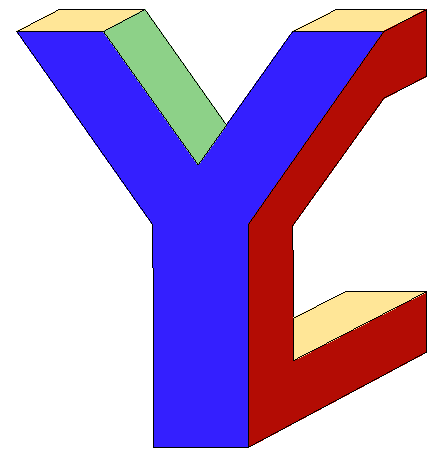
\includegraphics[height=1.5cm]{pictures/YC_logo.pdf}
    \end{center} 
  \end{tabular}
  \titlepage
\end{frame}
}

\begin{frame}[fragile]
  \transwipe[direction=90]
  \frametitle{YaccConstructor}
  \begin{itemize}
    \item Исследования в области формальных языков и синтаксического анализа
    \item Исследовательские задачи
    \item Открытый исходный код
    \begin{itemize}
      \item \url{https://github.com/YaccConstructor}
    \end{itemize}
    \item F\# --- основной язык разработки
    \begin{itemize}
      \item А также Coq, Haskel $\dots$
    \end{itemize}
  \end{itemize}
\end{frame}

\begin{frame}[fragile]
  \transwipe[direction=90]
  \frametitle{Области интересов}
  \begin{itemize}
    \item Граммтики, другие способы формализации языков
    \item Поиск путей в графах с ограничениями, выраженными в терминах языков
    \begin{itemize}
      \item Статический анализ кода
      \item Графовые базы данных
    \end{itemize}
    \item Вывод грамматик (grammar inference)
  \end{itemize}
\end{frame}

\begin{frame}[plain,c]
 \transwipe[direction=90]
 \begin{center}
  \Huge Задачи
 \end{center}
\end{frame}

\begin{frame}
  \transwipe[direction=90]
  \frametitle{Пересечение контекстно-свободных граммтик}
  \begin{itemize}
    \item Руководитель: Семён Григорьев (\url{rsdpisuy@gmail.com})
    \item \textbf{Задача.} Существует алгоритм пересечения произвольной и нерекурсивной КС грамматик, основанный на алгоритме синтаксического анализа CYK. 
    Необходимо выяснить, можно ли построить алгоритм для решения этой задачи, основанный на матричных операциях. Если такое возможно, то предъявить этот алгоритм.   
    \item Подробное описание задачи: \url{https://goo.gl/WKbCSo}
  \end{itemize}
\end{frame}

\begin{frame}
  \transwipe[direction=90]
  \frametitle{Восстановление после ошибок}
  \begin{itemize}
    \item Руководитель: Семён Григорьев (\url{rsdpisuy@gmail.com})
    \item \textbf{Задача.} Реализовать алгоритм восстановления после ошибок, основанный на синтаксическом анализе графов, и провести его экспериментальное исследование.
    В рамках экспериментального исследования необходимо реализовать граммтику одного или нескольких языков программирования (C\#, Java и т.д.).
    \item Подробное описание задачи: \url{https://goo.gl/JB5brY}
  \end{itemize}
\end{frame}

\begin{frame}
  \transwipe[direction=90]
  \frametitle{Конъюнктивный синтаксический анализ графов}
  \begin{itemize}
    \item Руководитель: Рустам Азимов (\url{rustam.azimov19021995@gmail.com})
    \item \textbf{Задача.} 
    Существует алгоритм синтаксического анализа графов для линейных конъюнктивных грамматик. 
    В нашей лаборатории разработан алгоритм синтаксического анализа графов, работающий с произвольной конъюнктивной грамматикой.
    Требуется реализовать его и провести сравнение с алгоритмом для линейных конъюнктивных грамматик. 
    Для проведения сравнения необходимо подготовить входные данные: графы и грамматики.
    \item Подробное описание задачи: \url{https://goo.gl/hqv1Xi}
  \end{itemize}
\end{frame}

\begin{frame}
  \transwipe[direction=90]
  \frametitle{Конъюнктивные и конъюнктивные контекстно-свободные запросы}
  \begin{itemize}
    \item Руководитель: Рустам Азимов (\url{rustam.azimov19021995@gmail.com})
    \item \textbf{Задача.} 
    Существует два типа запросов к графам: конъюнктивные контекстно-свободные и конъюнктивные. 
    Требуется найти соотношение между этими двуя типами.
    Наша гипотеза: конъюнктивные контекстно-свободные включаются в конъюнктивные.
    В качестве первого шага можно попробовать доказать или опровергнуть её. 
    Если гипотеза окажется верной, то необходимо построить алгоритм преобразоватния конъюнктивных контекстно-свободных запросов в конъюнктивные.
    \item Подробное описание задачи: \url{https://goo.gl/LUnyJo}
  \end{itemize}
\end{frame}


\begin{frame}
  \transwipe[direction=90]
  \frametitle{Попарсить GitHub!}
  \begin{itemize}
    \item Руководитель: Артём Горохов
    \item \textbf{Задача.}
    В YaccConstructor реализовано несколько алгоритмов синтаксического анализа. Хотелось бы сравнить их работу на различных данных. Для этого предлагается написать грамматики для 3-4 известных языков программирования и парсить код из репозиториев на GitHub.
    \item Подробное описание задачи: \url{https://goo.gl/BFXXnZ}
  \end{itemize}

\end{frame}

            
\begin{frame}
\transwipe[direction=90]
\frametitle{Контакты}
\begin{itemize}
  \item Семён Григорьев: \url{rsdpisuy@gmail.com}
  \item Артём Горохов: \url{gorohov.art@gmail.com}
  \item Рустам Азимов: \url{rustam.azimov19021995@gmail.com}
  \item Исходный код YaccConstructor: \url{https://github.com/YaccConstructor}
\end{itemize}
\end{frame}
\end{document}
